\documentclass{beamer}
\usetheme{Antibes}

\usepackage[makeroom]{cancel}
\usepackage{graphicx}
\usepackage{esvect}
\usepackage{xcolor}
\usepackage{tabularx}

\def\*#1{\mathbf{#1}}
\def\rr{\rightarrow}
\newcommand{\norm}[1]{\left\lVert#1\right\rVert}
\usefonttheme[onlymath]{serif}

\title[curvature]{Discrete Curvature Computation\\ \small{work report}}
\author{MinliangLIN}
\date{\tiny\today}

\begin{document}
\frame{\titlepage}

\begin{frame}
  \frametitle{Outline}
  \tableofcontents
\end{frame}

\section{Review}
\frame{{Review}
\begin{itemize}
  \item $X$ is a tangent vector of the surface, $B$ is a $2\times 2$ matrix.
  \item Normal curvature is a quadratic form of tangent vector $X^TBX$.
  \item $B$ is called curvature tensor.
\end{itemize}
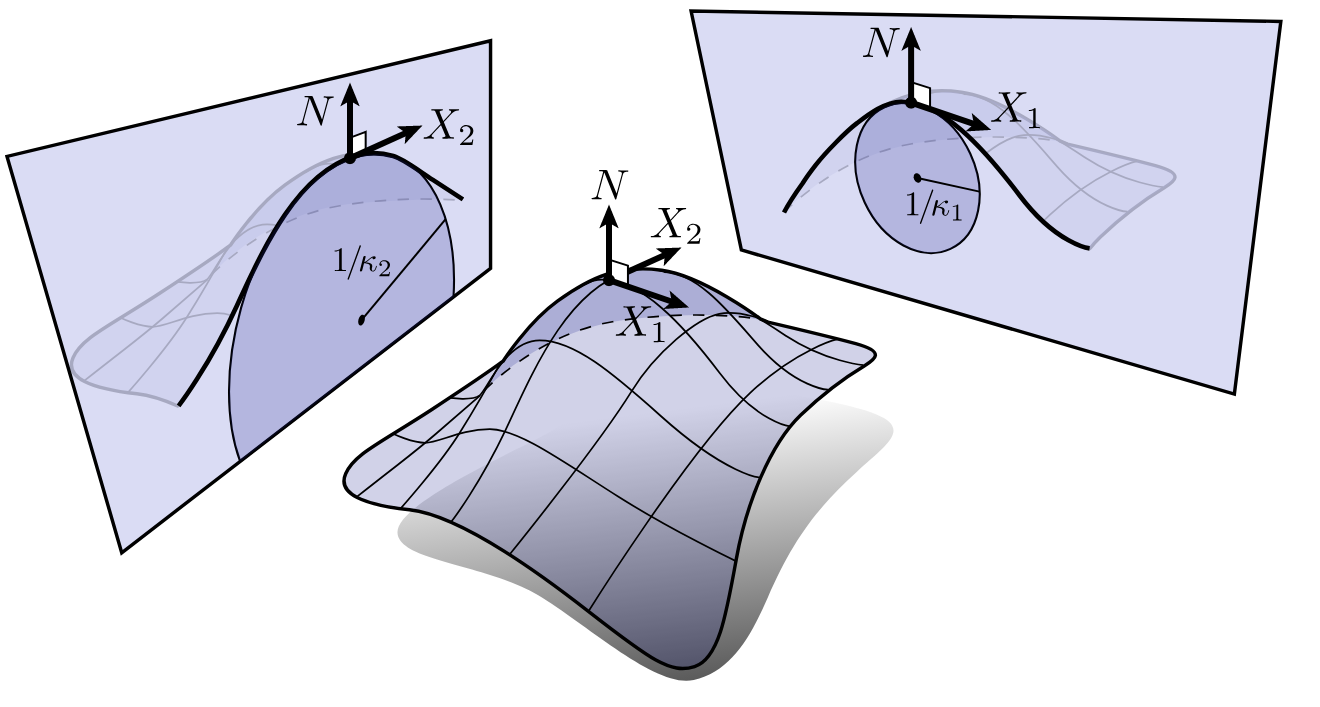
\includegraphics[width=0.5\textwidth]{../img/principal}
}

\frame{{Review}
\begin{itemize}
  \item $\kappa_H = \frac{1}{2}tr(B)$ is called mean curvature
  \item $\kappa_G = \det(B)$ is called Gauss curvature
  \item Last time, we use \textit{Discrete Geometry Operator}, which computes
  \begin{itemize}
    \item $\kappa_H$ by linear combination of coordinate of vertices of 1-ring,
    \item $\kappa_G$ by angular defect, and
    \item $B$ by least square.
  \end{itemize}
\end{itemize}
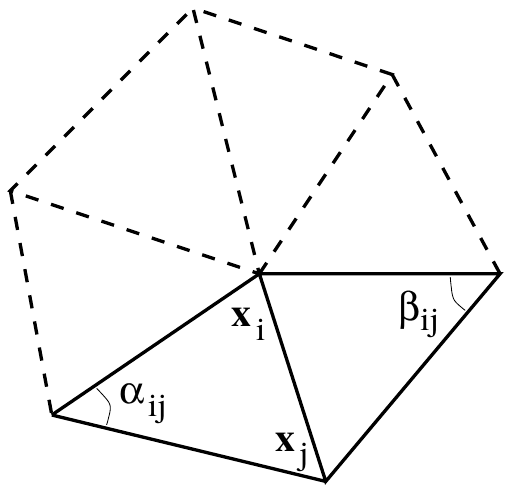
\includegraphics[width=0.3\textwidth]{../img/star}
}

\section{Issues}
\frame{{Targets}
We want the curvature to be
\begin{itemize}
  \item tessellation independent,
  \item feature-and-boundary aware, and
  \item adjustable radius of neighbourhood.
\end{itemize}
}

\frame{{Issues}
For example, angular defect method may not converge. Known sufficient condition are:
\begin{itemize}
  \item vertex valence is 6, or
  \item the valence is 4 with the one-ring neighbours are aligned with the principal directions.
\end{itemize}
\includegraphics<1>[width=0.5\textwidth]{../img/gauss}
\includegraphics<2>[width=0.7\textwidth]{../img/converge}
}

\frame{{Issues}
If you are doing least square wrongly...
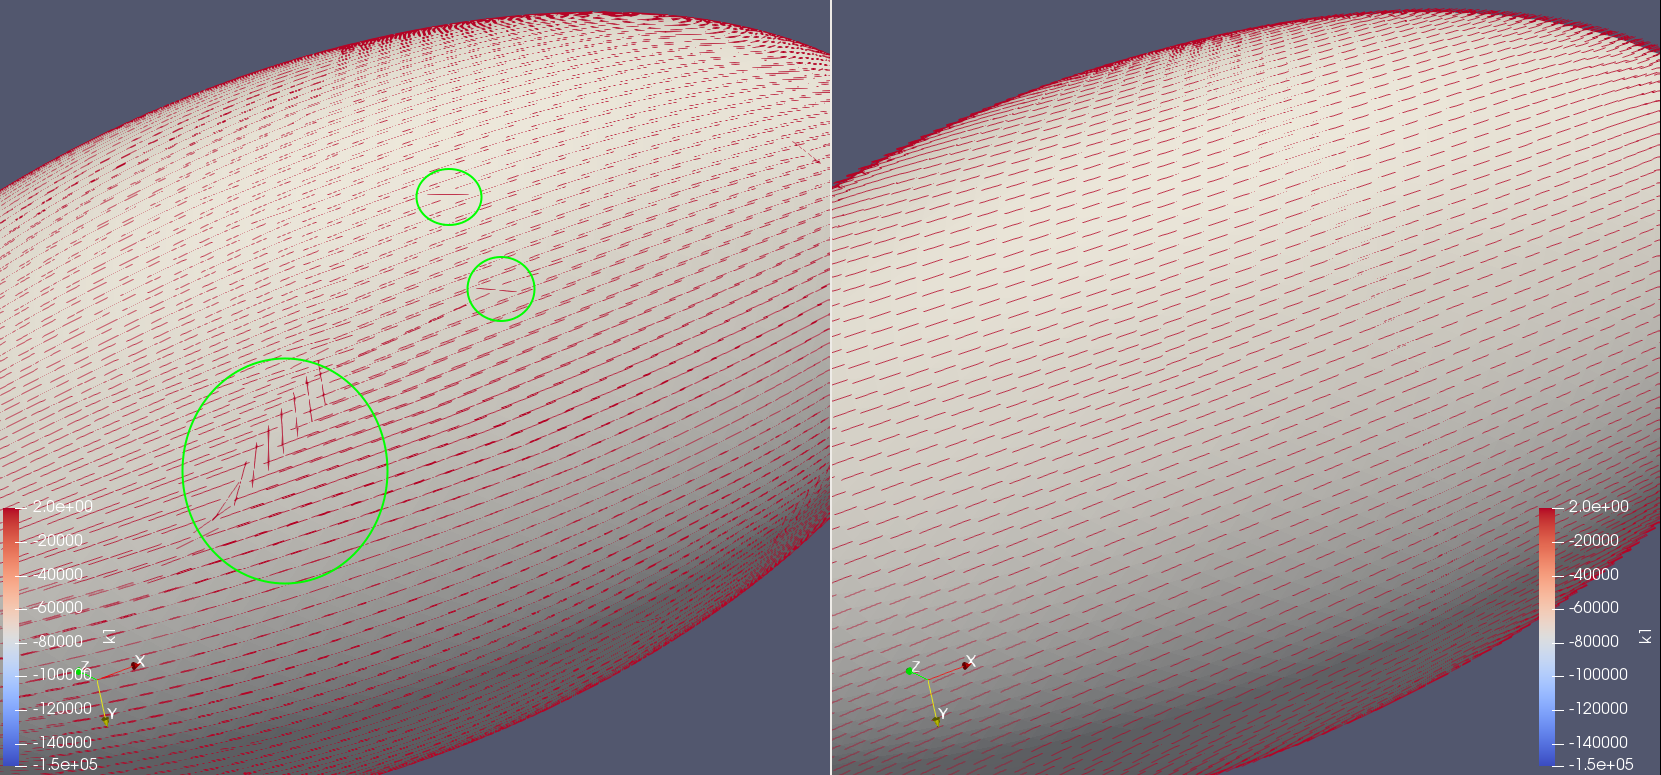
\includegraphics[width=\textwidth]{../img/lsq}
}

\section{Other methods}

\frame{{Normal cycle}
Normal cycle: a kind of non-linear interpolation.
\[
B = \sum_{e\in E}\beta(e)length(e)\vec{e}\otimes\vec{e}
\]
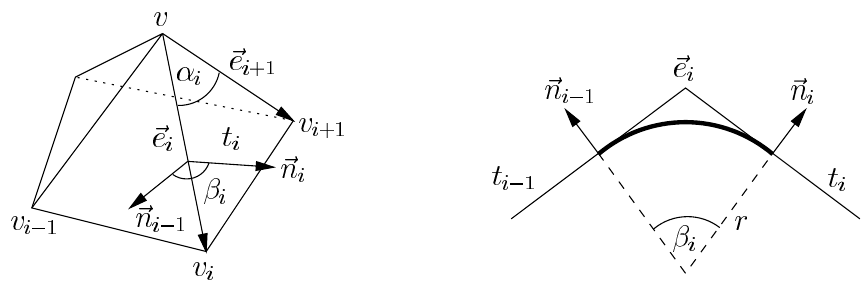
\includegraphics[width=0.8\textwidth]{../img/nc}
}

\frame{{Fitting}
Polynomial fitting method consists of the following steps:
\begin{itemize}
  \item Use BFS to gather enough vertexes in the ball of radius $r$.
  \item Set a local frame.
  \item Express gathered data in the local frame and fitting a polynomial.
  \item Evaluate the curvature tensor.
\end{itemize}
}

\frame{{Reference}

\begin{table}[h]\tiny
\begin{tabularx}{\textwidth}{p{4em} | p{3.5em} | X | X}\hline
name & paper & implementation & curvature species \\ \hline
discrete geometry operator & \cite{meyer2003discrete} & VCG::MeanAndGaussian & mean curvature and gaussian curvature \\ \hline
normal cycle  & \cite{cohen2003restricted} \cite{dyn2001optimizing} & VCG::PrincipalDirectionsNormalCycle and VCG::ComputeSingleVertexCurvature &  mean curvature, gaussian curvature and principal curvature and principal direction  \\ \hline
polynomial fitting  & \cite{cazals2005estimating} \cite{panozzo2010efficient} & CGAL::Monge\_via\_jet\_fitting::Monge\_form, IGL::principal\_curvature & mean curvature, gaussian curvature and principal curvature and principal direction \\  \hline
tensor fitting  & \cite{meyer2003discrete} \cite{taubin1995estimating} & VCG::PrincipalDirections & principal curvature and principal direction \\ \hline
PCA estimation  & \cite{yang2006robust} & VCG::PrincipalDirectionsPCA & principal curvature and principal direction \\ \hline
\end{tabularx}
\end{table}

}

\frame{{Reference}\small
\bibliography{bib}
\bibliographystyle{alpha}
}

\end{document}
